\documentclass[10pt,onecolumn]{IEEEtran}
\input{preamble.tex}

% Standalone build: do not require shell escape.
\tikzexternaldisable
\pgfplotsset{compat=1.18}
\newif\iftikzX
\tikzXtrue


\begin{document}
\pagestyle{empty}

\begin{figure}
\tikzexternalenable 
  \tikzsetnextfilename{figres}
  \centering
   \iftikzX   
  % The boxplot command below exposes all visible components directly.
% PGFPlots computes quartiles and 1.5-IQR whiskers from the raw CSV column;
% no mean marker is drawn.
\newcommand{\ControlledBoxPlot}[4]{%
  \addplot[
    boxplot/draw direction=y,
    boxplot={
      draw position=#1,
      box extend=0.37,
      whisker range=2.5
    },
    draw=#2,
    fill=#2!9,
    line width=0.55pt,
    boxplot/every box/.style={draw=#2, fill=#2!9, line width=0.55pt},
    boxplot/every whisker/.style={draw=#2, line width=0.50pt},
    boxplot/every median/.style={draw=black, line width=0.85pt},
    mark=o,
    mark size=1.2pt,
    mark options={draw=#2, fill=white, line width=0.35pt}
  ] table[y=#4, col sep=comma] {#3};%
}
% Data files.
\newcommand{\WaveLSM}{data/wave_lsm.csv}
\newcommand{\WaveChow}{data/wave_chow_liu.csv}
\newcommand{\WaveCTGAN}{data/wave_ctgan.csv}
\newcommand{\WaveBase}{data/wave_baseline.csv}
\newcommand{\WaveCtrl}{data/wave_original_sample_control.csv}
\newcommand{\SumLSM}{data/summary_lsm.csv}
\newcommand{\SumChow}{data/summary_chow_liu.csv}
\newcommand{\SumCTGAN}{data/summary_ctgan.csv}
\newcommand{\SumBase}{data/summary_baseline.csv}
\newcommand{\SumCtrl}{data/summary_original_sample_control.csv}

% Consistent generator colors.
\definecolor{lsmcol}{RGB}{31,119,180}
\definecolor{chowcol}{RGB}{230,126,34}
\definecolor{ctgancol}{RGB}{46,139,87}
\definecolor{basecol}{RGB}{192,57,43}
\definecolor{ctrlcol}{RGB}{117,107,177}

\begin{tikzpicture}[font=\sffamily\fontsize{7}{8}\selectfont]
  \def\OPC{.60}
\begin{groupplot}[
  group style={group size=2 by 2, horizontal sep=0.62in, vertical sep=0.75in},
  width=1.65in,
  height=1.30in,
  scale only axis=true,
  axis line style={draw=black!75, line width=0.45pt},
  tick style={draw=black!65, line width=0.35pt},
  tick align=outside,
  major tick length=2pt,
  %tick label style={font=\scriptsize},
  %label style={font=\scriptsize},
  %title style={%font=\footnotesize,
 %   yshift=1pt},
  grid=major,
  major grid style={draw=black!10, line width=0.30pt},
  minor tick num=0,    major tick length=0pt,
  scaled ticks=false,
  enlargelimits=false,
  %title style={yshift=-.1in},
]

% ------------------------------------------------------------------
% (a) MAP-alignment--novelty frontier.
% Labels are attached to the plotted points by nodes near coords;
% no axis coordinates are repeated in separate \node commands.
% ------------------------------------------------------------------
\nextgroupplot[
  title={(a) Excess alignment--novelty frontier},
  xlabel={Mean row novelty},
  ylabel={Excess MAP-alignment fraction $\Lambda$},
  xmin=-0.025, xmax=0.67,
  ymin=-0.08, ymax=1.20,
  xtick={0,0.2,0.4,0.6},
  ytick={0,0.25,0.50,0.75,1.00},
]
% Independence null: Lambda = 0.
%\addplot[black!55, dashed, thin, no marks, forget plot]
 % coordinates {(-0.025,0) (0.67,0)};

% Original-row reference: Lambda = 1.
%\addplot[black!55, solid, thin, no marks, forget plot]
%  coordinates {(-0.025,1) (0.67,1)};
\addplot[
  only marks, mark=*, mark size=1.85pt, lsmcol,
  error bars/.cd, x dir=both, y dir=both, x explicit, y explicit,
  error bar style={opacity=\OPC,line width=0.55pt},
  error mark options={rotate=90, mark size=1.5pt, line width=0.55pt},
  /pgfplots/.cd,
  nodes near coords={LSM},
  nodes near coords style={font=\scriptsize, text=lsmcol, anchor=east, xshift=-2pt, yshift=1pt}
] table[
  x=mean_row_novelty, y=mean_excess_alignment,
  x error plus expr=\thisrow{novelty_bootstrap_ci_high}-\thisrow{mean_row_novelty},
  x error minus expr=\thisrow{mean_row_novelty}-\thisrow{novelty_bootstrap_ci_low},
  y error plus expr=\thisrow{excess_alignment_ci_high}-\thisrow{mean_excess_alignment},
  y error minus expr=\thisrow{mean_excess_alignment}-\thisrow{excess_alignment_ci_low},
  col sep=comma
] {\SumLSM};

\addplot[
  only marks, mark=square*, mark size=1.70pt, chowcol,
  error bars/.cd, x dir=both, y dir=both, x explicit, y explicit,
  error bar style={line width=0.55pt},
  error mark options={rotate=90, mark size=1.5pt, line width=0.55pt},
  /pgfplots/.cd,
  nodes near coords={Chow--Liu},
  nodes near coords style={font=\scriptsize, text=chowcol, anchor=west, xshift=2pt, yshift=-2pt}
] table[
  x=mean_row_novelty, y=mean_excess_alignment,
  x error plus expr=\thisrow{novelty_bootstrap_ci_high}-\thisrow{mean_row_novelty},
  x error minus expr=\thisrow{mean_row_novelty}-\thisrow{novelty_bootstrap_ci_low},
  y error plus expr=\thisrow{excess_alignment_ci_high}-\thisrow{mean_excess_alignment},
  y error minus expr=\thisrow{mean_excess_alignment}-\thisrow{excess_alignment_ci_low},
  col sep=comma
] {\SumChow};

\addplot[
  only marks, mark=triangle*, mark size=1.85pt, ctgancol,
  error bars/.cd, x dir=both, y dir=both, x explicit, y explicit,
  error bar style={line width=0.55pt},
  error mark options={rotate=90, mark size=1.5pt, line width=0.55pt},
  /pgfplots/.cd,
  nodes near coords={CTGAN},
  nodes near coords style={font=\scriptsize, text=ctgancol, anchor=west, xshift=2pt, yshift=2pt}
] table[
  x=mean_row_novelty, y=mean_excess_alignment,
  x error plus expr=\thisrow{novelty_bootstrap_ci_high}-\thisrow{mean_row_novelty},
  x error minus expr=\thisrow{mean_row_novelty}-\thisrow{novelty_bootstrap_ci_low},
  y error plus expr=\thisrow{excess_alignment_ci_high}-\thisrow{mean_excess_alignment},
  y error minus expr=\thisrow{mean_excess_alignment}-\thisrow{excess_alignment_ci_low},
  col sep=comma
] {\SumCTGAN};

\addplot[
  only marks, mark=diamond*, mark size=1.75pt, basecol,
  error bars/.cd, x dir=both, y dir=both, x explicit, y explicit,
  error bar style={line width=0.55pt},
  error mark options={rotate=90, mark size=1.5pt, line width=0.55pt},
  /pgfplots/.cd,
  nodes near coords={Independent},
  nodes near coords style={font=\scriptsize, text=basecol, anchor=east, xshift=-2pt, yshift=-2pt}
] table[
  x=mean_row_novelty, y=mean_excess_alignment,
  x error plus expr=\thisrow{novelty_bootstrap_ci_high}-\thisrow{mean_row_novelty},
  x error minus expr=\thisrow{mean_row_novelty}-\thisrow{novelty_bootstrap_ci_low},
  y error plus expr=\thisrow{excess_alignment_ci_high}-\thisrow{mean_excess_alignment},
  y error minus expr=\thisrow{mean_excess_alignment}-\thisrow{excess_alignment_ci_low},
  col sep=comma
] {\SumBase};

\addplot[
  only marks, mark=*, mark size=1.65pt, ctrlcol,
  error bars/.cd, x dir=both, y dir=both, x explicit, y explicit,
  error bar style={line width=0.50pt},
  error mark options={rotate=90, mark size=1.4pt, line width=0.50pt},
  /pgfplots/.cd,
  nodes near coords={Original (control)},
  nodes near coords style={font=\scriptsize, text=ctrlcol, anchor=west, xshift=2pt, yshift=2pt}
] table[
  x=mean_row_novelty, y=mean_excess_alignment,
  x error plus expr=\thisrow{novelty_bootstrap_ci_high}-\thisrow{mean_row_novelty},
  x error minus expr=\thisrow{mean_row_novelty}-\thisrow{novelty_bootstrap_ci_low},
  y error plus expr=\thisrow{excess_alignment_ci_high}-\thisrow{mean_excess_alignment},
  y error minus expr=\thisrow{mean_excess_alignment}-\thisrow{excess_alignment_ci_low},
  col sep=comma
] {\SumCtrl};

% ------------------------------------------------------------------
% (b) Signed MAP-alignment gap. No mean triangles are drawn.
% Boxes show Q1--Q3, black line is median, whiskers use 1.5 IQR,
% and open circles are points beyond the whiskers.
% ------------------------------------------------------------------
\nextgroupplot[
  title={(b) Signed MAP-alignment gap},
  ylabel={$\Upsilon_{\mathrm{syn}}-\Upsilon_{\mathrm{control}}$},
  xmin=0.55, xmax=4.45,
  ymin=-0.075, ymax=0.045,
  xtick={1,2,3,4},
  xticklabels={LSM,Chow--Liu,CTGAN,Independent},
  x tick label style={rotate=25, anchor=east,yshift=-.05in},
  ytick={-0.06,-0.04,-0.02,0,0.02,0.04},
  yticklabel style={/pgf/number format/fixed,/pgf/number format/precision=2},
]
\ControlledBoxPlot{1}{lsmcol}{\WaveLSM}{signed_gap_vs_control}
\ControlledBoxPlot{2}{chowcol}{\WaveChow}{signed_gap_vs_control}
\ControlledBoxPlot{3}{ctgancol}{\WaveCTGAN}{signed_gap_vs_control}
\ControlledBoxPlot{4}{basecol}{\WaveBase}{signed_gap_vs_control}
\addplot[black!55, thin, no marks, forget plot] coordinates {(0.55,0) (4.45,0)};

% ------------------------------------------------------------------
% (c) Row novelty. Same explicit box construction.
% ------------------------------------------------------------------
\nextgroupplot[
  title={(c) Row novelty across waves},
  ylabel={Row novelty},
  xmin=0.55, xmax=5.45,
  ymin=-0.025, ymax=0.68,
  xtick={1,2,3,4,5},
  xticklabels={LSM,Chow--Liu,CTGAN,Independent,Original (control)},
  x tick label style={rotate=25, anchor=east,yshift=-.05in},
  ytick={0,0.2,0.4,0.6},
]
\ControlledBoxPlot{1}{lsmcol}{\WaveLSM}{row_novelty}
\ControlledBoxPlot{2}{chowcol}{\WaveChow}{row_novelty}
\ControlledBoxPlot{3}{ctgancol}{\WaveCTGAN}{row_novelty}
\ControlledBoxPlot{4}{basecol}{\WaveBase}{row_novelty}
\ControlledBoxPlot{5}{ctrlcol}{\WaveCtrl}{row_novelty}

% ------------------------------------------------------------------
% (d) Wave-wise retention.
% ------------------------------------------------------------------
\nextgroupplot[
  title={(d) Wave-wise MAP-alignment retention},
  xlabel={GSS wave [year]},
  ylabel={$\Upsilon_{\mathrm{synthetic}}/\Upsilon_{\mathrm{control}}$},
  xmin=1972, xmax=2024,
  ymin=0.905, ymax=1.055,
  xtick={1972,1980,1990,2000,2010,2020},
  xticklabel style={/pgf/number format/1000 sep=},
  ytick={0.92,0.96,1.00,1.04},
  legend style={font=\scriptsize, at={(0.02,1.01)}, anchor=north west,
    draw=none, fill=none, legend columns=2,
    /tikz/every even column/.append style={column sep=4pt}},
]
\addplot[lsmcol, opacity=\OPC,smooth, mark=*, mark size=0.95pt, line width=0.65pt]
  table[x=year, y=fidelity_retention, col sep=comma] {\WaveLSM};
\addlegendentry{LSM}
\addplot[chowcol, opacity=\OPC,smooth,mark=square*, mark size=0.90pt, line width=0.65pt]
  table[x=year, y=fidelity_retention, col sep=comma] {\WaveChow};
\addlegendentry{Chow--Liu}
\addplot[ctgancol, opacity=\OPC,smooth,mark=triangle*, mark size=1.00pt, line width=0.65pt]
  table[x=year, y=fidelity_retention, col sep=comma] {\WaveCTGAN};
\addlegendentry{CTGAN}
\addplot[basecol, opacity=\OPC,smooth,mark=diamond*, mark size=0.95pt, line width=0.65pt]
  table[x=year, y=fidelity_retention, col sep=comma] {\WaveBase};
\addlegendentry{Ind. baseline}
\addplot[black!55, thin, no marks, forget plot] coordinates {(1972,1) (2024,1)};

\end{groupplot}
\end{tikzpicture}

  \else
  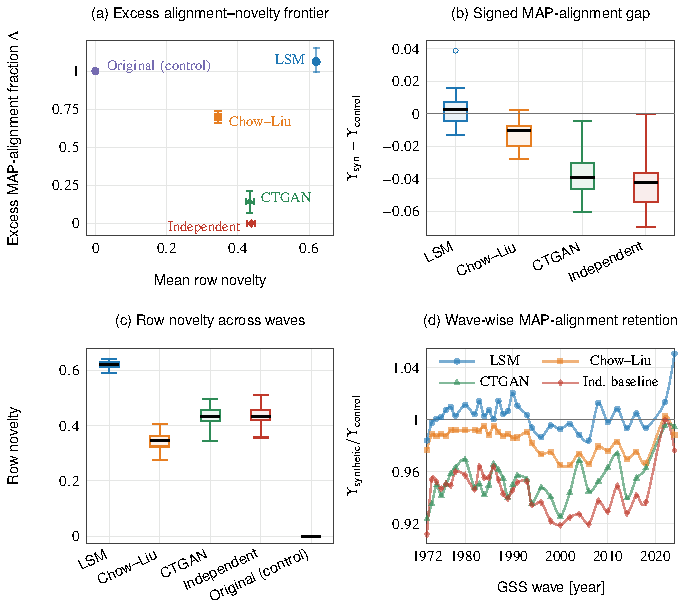
\includegraphics[width=.35\textwidth]{Figures/External/figres}
  \fi

\caption{Four complementary views of the GSS benchmark. (a) Cross-wave MAP-alignment--novelty frontier with nonparametric 95\% wave-bootstrap intervals. (b) Wave-level signed MAP-alignment differences from the original-row control. (c) Wave-level row novelty, defined as one minus mean nearest-real similarity. (d) MAP-alignment retention by GSS wave. The label ``Chow--Liu'' denotes the restricted Chow--Liu hybrid.}
\label{fig:gss_benchmark_four_panel}
\end{figure}

\end{document}
